\newpage

\begin{appendices}

\section{EIP-1729. Introduce SQL semantics to EVM <WIP>}
We are contemplating an EIP (Ethereum Improvement Proposal) to give Ethereum dapp developers a new choice for data storage. Not all data need to be replicated on every full node of Ethereum as the need for strongest security maybe an overkill for most smart contracts. Such data can be stored on \textsf{Picolo} network at a contract defined replication factor. Specifically, the EIP plans to introduce SQL primitives like selections, projections, aggregates etc directly into solidity (feasibility currently being evaluated).
\newline
\newline
\textsf{Picolo} may also be used by ``stateless clients'' and ``state minimized clients'' to query for data that is normally hosted by ``archival nodes'' in the current implementation or in the upcoming sharded implementation. \textsf{Picolo}'s SQL capabilities make it easy for clients to construct complex queries that are not currently possible in the simple key-value lookups provided by the EVM (Ethereum Virtual Machine).
\newline\newline
\texttt{<Mapping of SQL commands to EVM/eWASM opcodes to be defined here. Or maybe just a library contract or other ``listener'' mechanism will be easier to implement>}

\newpage
\section{Background on p2p networks} 
\label{appendix:p2p}

Since a fast production quality peer-peer network is a critical layer for any decentralized service architecture, we
present a summary of the past work in this area for educational purposes.

Napster \cite{Napster} was one of the first popular services that provided much of the original inspiration for p2p
systems although its database was centralized.  DNS is an example of a widely deployed distributed and largely
decentralized key-value database that powers every lookup and interaction on the Internet \cite{Mockapetris_1988}. DNS
relies on special root servers to bootstrap the lookup protocol. The Freenet \cite{freenet_thesis, Clarke_2001} and the
Gnutella \cite{Gnutella} p2p systems were popular in the previous decade for file sharing. Both systems were designed
for sharing of large files over a longer duration of time. Content reliabilty including lookup reliability and network
latency goals were necessary in this enviroment. 
\newline\newline
The second generation of p2p systems include research driven projects such as Chord \cite{Stoica_2001}, Content
Addressable Network (CAN)
\cite{Ratnasamy_2001}, Pastry \cite{Rowstron_2001}, Tapestry \cite{tapestry2004} and
Kademlia. Chord along with CAN, Tapestry and Pastry developed the concept of distributed hash tables (DHTs) as a
fundamental mechanism for content-based addressing. They built over the scalability and self-organizing properties of
both FreeNet and Gnutella by providing a definite answer to a lookup query in a bounded number of network hops. In fact,
these protocols are able to locate content within \( O(log N) \) where \(N\) is the number of nodes in the system. From
an 
API perspective, these overlays provide a key-based routing (KBR) interface that supports deterministic routing of
messages to a live node that has the responsiblity for the ``value'' corresponding to the given key. These systems also
support high level APIs such as Dynamic Object Location and Routing (DOLR) \cite{dolr2003}. Most DHT's use the concept
of consistent hashing to distribute load evenly among the nodes. Consistent hashing refers to a technique which
creates `buckets' of items such that a small change in the buckets does not lead to a large amount of rehashing.
\newline\newline
% {\em Consistent hashing:}
% Typical hashing based schemes do a good job of spreading load through a known, fixed collection of servers. Since the
% Blockchain consists of nodes on the Internet which can appear and disappear based on incentives and other criteria, our
% assumption is that machines come and go as they crash or are brought into the network. Also,
% the information about what nodes are functional propagates slowly through the
% network, so that clients may have incompatible “views” of which nodes are available to replicate data. (Note that a
% node can also be a client). This makes standard hashing useless since it relies on clients agreeing on which nodes are responsible for serving a particular
% page.
% 
% Like most hashing schemes, consistent hashing assigns a set of items to buckets so that
% each bin receives roughly the same number of items.  Unlike standard hashing schemes, a small change in the bucket set
% does not induce a total remapping of items to buckets. In addition, hashing items into slightly different sets of
% buckets gives only slightly different assignments of items to buckets. 
% 
Chord uses such hash functions to map nodes and content uniformly to a circular 160-bit
namespace. Chord improves the scalability of consistent hashing by removing the requirement that every node knows about
every other node. Each node only maintains about \(O (log N) \) state information about other nodes in an \( N \) node
network. When nodes join or leave, they require \( O(log^2 N) \) messages to keep the network updated. CAN routes messages in a {\em d}-dimensional space where each node maintains a routing table with \(O(d)\) entries and
any node can be reached in \(O(dN^{1/d})\) routing hops. CAN's routing table does not grow with network size, but the
number of routing hops grows faster than \(log N\). When compared to Chord and CAN, Pastry and Tapestry take network distances into account when constructing overlay
topologies. While Chord and CAN use shortest overlay hops and other runtime heuristics, both Tapestry and Pastry
construct locally optimal routing tables to reduce any routing inefficiencies. 
\newline\newline
Pastry and Tapestry share some similarities to the work by Plaxton et al \cite{Plaxton_1997} and to the routing layer in
the Landmark hierarchy \cite{Tsuchiya_1988}. The approach consists of routing based on address prefixes or otherwise
called prefix-based routing. However, both Pastry and Tapestry include an ability to self-organize the network structure
and achieve network locality in content mapping which also lends support for replication.
In addition, Tapestry also allows some application-based locality management by "publishing" location pointers
throughout the network for efficiently locating content and services.
\newline\newline
Kademlia \cite{kademlia} is another p2p DHT-based routing system that uses prefix-based routing by arranging 160-bit IDs
(node IDs and content IDs) in a binary tree style data-structure for efficient routing. It uses an XOR-based distance
metric for building the routing table and for the routing algorithm itself. In terms of its performance and other
features, it is very similar to the above systems such as Chord, CAN, Pastry and Tapestry, but it offers simplicity in
its routing and lookup algorithms which make it attrative for implementation. IPFS \cite{ipfs} uses a version of
Kademlia for locating files for decentralized applications.
\newline\newline
Other notable systems include Viceroy \cite{viceroy} which provides logarithmic hops through nodes with constant degree
routing tables. SkipNet \cite{skipnet} uses a multidimensional skip-list data structure to support overlay routing,
maintaining both a DNS-based namesapce for operational locality and a randomized namespace for network locality. Other
overlay proposals such as Koorde \cite{koorde} and Naor et al \cite{simple_hash} attain lower bounds on local routing
state but oversimplify some of the other features. 
\newline\newline
The third generation of p2p research includes building applications on top of these DHT systems, validating them as
novel infrastructures or tuning them for specific use cases. For example, applications such as PAST \cite{past} and
SCRIBE \cite{scribe} are built on top of Pastry. Decentralized file storage application project OceanStore \cite{oceanstore} was built
on top of Tapestry, while CFS \cite{cfs} was build on top of Chord. FarSite \cite{farsite} uses a conventional
distributed directory service and could be built on top of Pastry. Another example of an overlay network is the Overcast
System \cite{overcast}, which provides reliable single-source multicast streams.


\section{MX Protocol} \label{sec:mx_protocol}
Nodes in the network need to speak the same language for efficient discovery and communication of data. Hence the following message exchange scheme (see \figref{fig:mx}) is proposed similar to \cite{Protocol_Spec}. Note that the exact mapping between the following messages and underlying transport protocol is not discussed here and may change depending on the final transport protocol chosen (\textsf{QUIC} vs \textsf{TCP})
\newline
\newline
\textbf{PUT}:  A \textsf{PUT} message contains the query to be run, an optional list of nodes to run the query against and an optional max number of hops (needed in case of an empty node list). This is used for creating or updating data in the system.
\newline
\newline
\textbf{GET}: A \textsf{GET} message contains the query to be run, max number of hops, the number of results to retrieve, the mode of retrieval (pull vs push) and a transaction identifier. Client sends this to a server to retrieve results that match the query. Parameters in \textsf{GET} can be varied depending on application needs - a streaming application may choose the push mode in which server pushes data to the client as it becomes available up until the specified number is met. A latency sensitive application may choose to retrieve a small number of results in a batch in one pull.
\newline
\newline
\textbf{SEND}: Servers respond to each \textsf{GET} message with one or more \textsf{SEND} messages with results. In pull mode, there is only one \textsf{SEND} message followed by an \textsf{END} message where as in push mode there are multiple \textsf{SEND} messages followed by an \textsf{END} message.
\newline
\newline
\textbf{END}: Servers send \textsf{END} messages to clients to indicate that they have finished sending all results in response to a particular \textsf{GET} message.
\newline
\newline
\textbf{CLOSE}: A client can send a \textsf{CLOSE} message to the server to indicate that it no longer is interested in the remaining query results and close the transaction. It doesn't have to wait until all the results are retrieved.
\newline
\newline
\textbf{OK}: Server sends this message to a client as a positive acknowledgment to a client's message.
\newline
\newline
\textbf{ERROR}: Server sends this message to a client as a negative acknowledgment to a client's message.
\begin{figure}[h!] \centering
	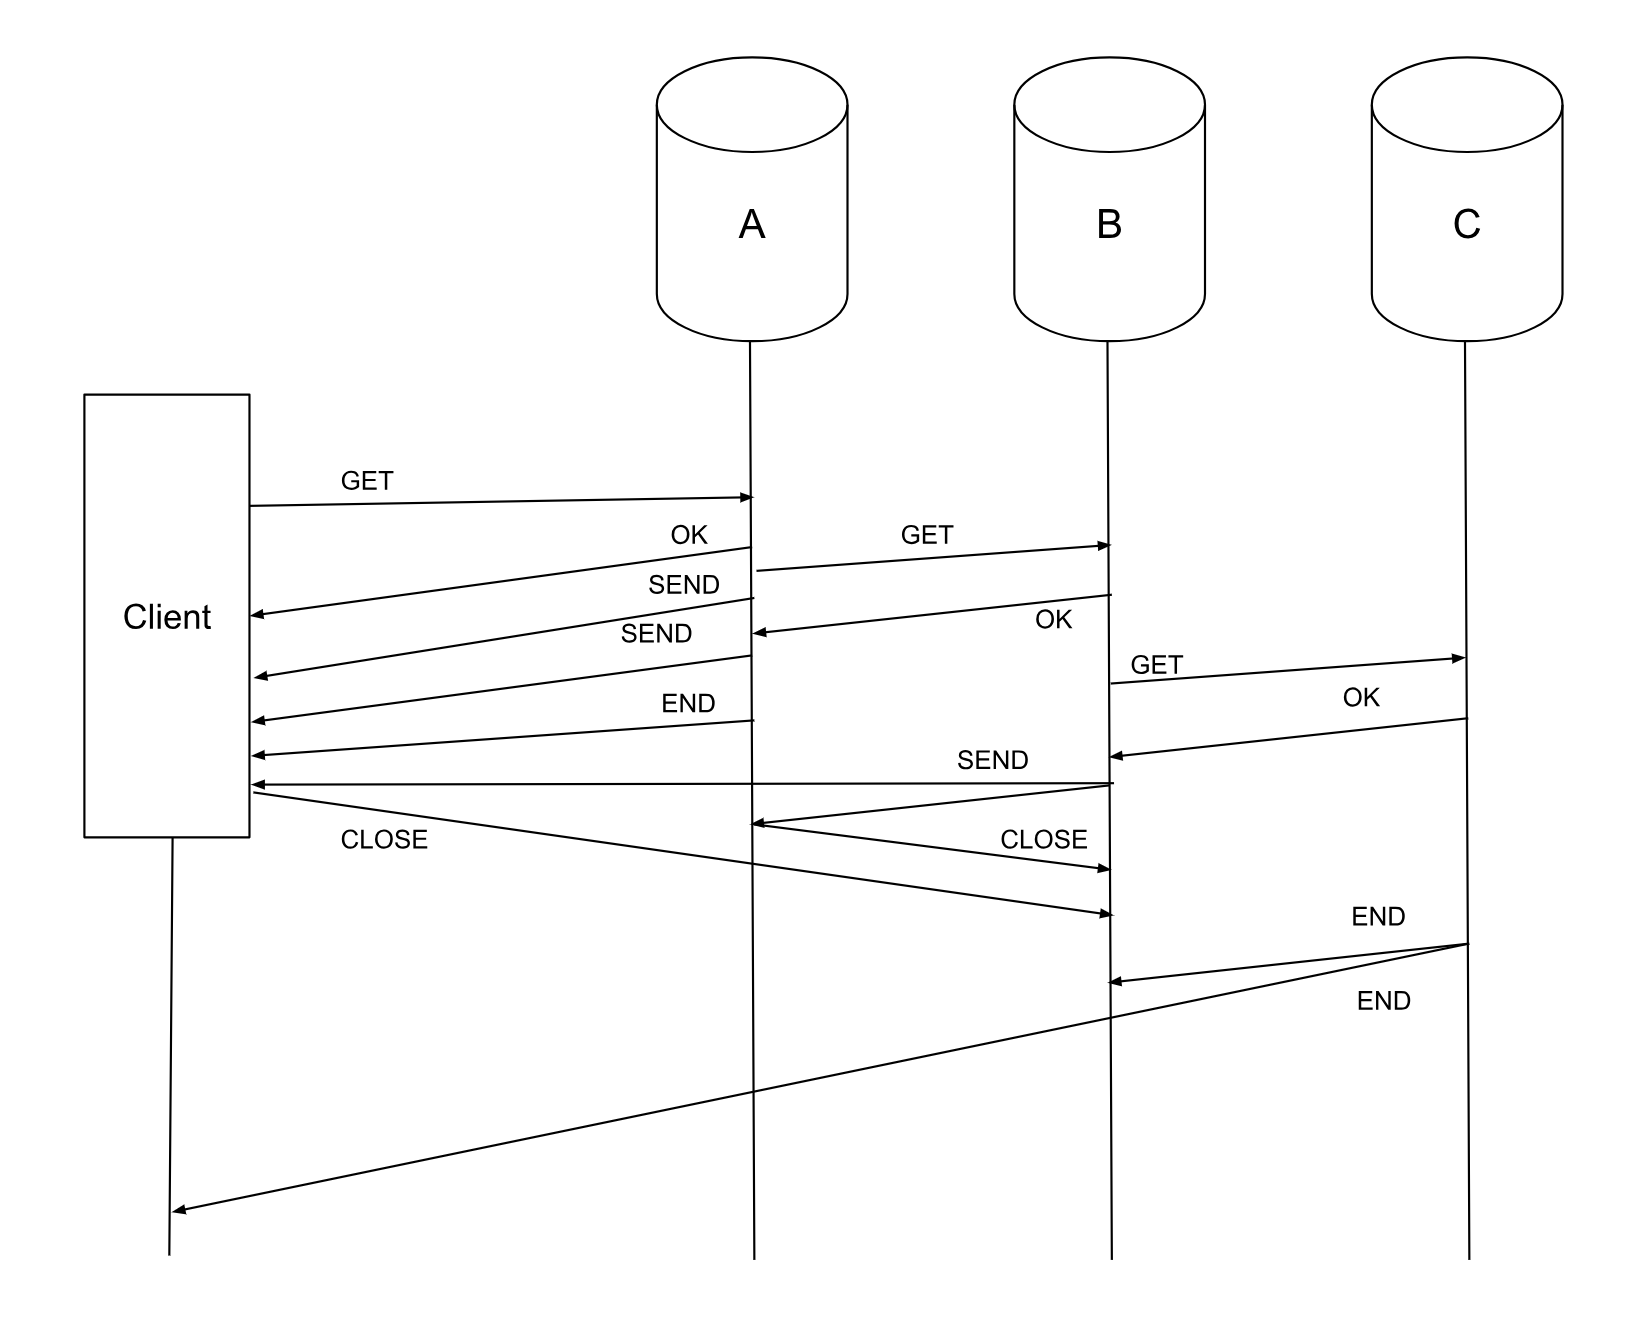
\includegraphics[width=\fscale{0.76}]{mx1.png}
	\caption{\textsf{GET} message flow, time increasing from top to bottom}
	\label{fig:mx}
\end{figure}



\end{appendices}
